% !TeX spellcheck = ru_RU
\documentclass[a4paper,11pt]{article}
\usepackage[process=auto]{pstool}
\usepackage[T2A]{fontenc}
\usepackage[utf8]{inputenc}
\usepackage[english,russian]{babel}
\usepackage{amssymb,amsmath}
\usepackage{gensymb,textcomp,latexsym}
\usepackage{graphicx}
\usepackage{tabularx}
\usepackage[pdftex, left=1in, right=1in, top=1in, bottom=2cm]{geometry}
\usepackage{parcolumns}
\usepackage{multirow}
\usepackage{tikz}

%\usepackage[usenames,dvipsnames]{xcolor}
%\usepackage[font=small,labelfont=bf]{caption}
%\usepackage[center]{subfigure}
%\renewcommand{\thesubfigure}{(\asbuk{subfigure})~}
\newcommand{\figref}[1]{Рис.~\ref{#1}}
%\usepackage[pdfauthor={Г. С. Щелик},pdftitle={Анализ поляризации дипольных волн в скважинах некругового сечения в анизотропной породе},pdfstartview=XYZ,bookmarks=true,colorlinks=true,linkcolor=blue,urlcolor=blue,citecolor=blue,bookmarks=true,linktocpage=true,hyperindex=true]{hyperref}
%\usepackage[hyperpageref]{backref}

%\usepackage[section]{placeins}
%\usepackage{graphicx}
%\usepackage{epsfig}
\usepackage{epstopdf}
%\usepackage{subfigure}
\usepackage{float}
%\floatstyle{boxed}
%\restylefloat{figure}
%\usepackage{booktabs}
%\graphicspath{ {./image_test/} }
%\usepackage{gs_trudy_based_style}

%%%

%%%

\newcommand{\ii}{\mathrm{i}}

\newcounter{modelnum}
\newcommand{\modelnum}[1]{\refstepcounter{modelnum}Модель \themodelnum #1}

%Filters counters
\newcounter{wfiltnum}
\newcommand{\wfiltnum}[1]{\refstepcounter{wfiltnum}ОФ-\thewfiltnum #1}
\newcounter{lffiltnum}
\newcommand{\lffiltnum}[1]{\refstepcounter{lffiltnum}НЧФ-\thelffiltnum #1}
\newcounter{hffiltnum}
\newcommand{\hffiltnum}[1]{\refstepcounter{hffiltnum}ВЧФ-\thehffiltnum #1}
%tabularx options
\newcolumntype{C}{>{\centering}X}



\begin{document}
\renewcommand\refname{\bfseries Литература}
%\part*{Анализ поляризации дипольных волн в скважинах некругового сечения в анизотропной породе}	

{\LARGE \bfseries \par \noindent Анализ поляризации дипольных волн в скважинах некругового сечения в анизотропной породе}
\par\bigskip

{\centering Г.С. Щелик$^{1,2}$ \par}
\medskip
{\centering \footnotesize
	$^1${Московский физико-технический институт} \par
	141700, Россия, Московская обл., г. Долгопрудный, Институтский пер., 9; \par
	$^2${Московский научный центр Шлюмберже} \par
	119285, Россия, г. Москва, ул. Пудовкина, 13; \par
	e-mail: german.schelik@phystech.edu,
	\par}
\par\bigskip

\par
%\affil[1]{Московский физико-технический институт}
%\affil[2]{Московский научный центр Шлюмберже}

\title{Анализ поляризации дипольных волн в скважинах некругового сечения в анизотропной породе}	
\begin{abstract}

Исследован вопрос определения главных направлений анизотропной породы в скважинах с нарушением цилиндрической геометрии с помощью численного моделирования измерений акустического каротажа. Модель используемых на практике алгоритмов обработки предполагает распространение вдоль скважины двух ортогонально поляризованных волн, которые в рассматриваемых задачах соответствуют дипольным модам. На примере эллиптических скважин показано, что направления колебаний мод могут быть существенно неортогональными и зависеть от частотного спектра сигнала источника, что приводит к некорректному определению главных направлений трансверсально-изотропной породы. Полученные после обработки направления сопоставлены с независимым расчётом собственных векторов дипольных мод полуаналитическим методом конечных элементов (SAFE). Результаты сравнения свидетельствуют об эффективности применения частотных фильтров и "неортогональных"\ алгоритмов для проверки корректности найденных направлений и повышения точности значений углов. %Приведённые в работе результаты имеют особую ценность для обработки каротажных измерений в наклонных и горизонтальных скважинах с деформациями ствола.
\end{abstract}

Ключевые слова: акустический каротаж, эллиптическая скважина, анизотропия, Alford rotation
\par

\section{Введение}
Последние несколько десятилетий в акустическом каротаже широко и достаточно успешно практикуются методики кросс-дипольных измерений. Современные решения в технике и обработке полученных данных позволяют производить количественную оценку азимутальной и аксиальной (по отношению к стволу скважины) анизотропии для широкой группы горных пород. Кросс-дипольные измерения также могут быть использованы для определения ориентации крупных трещин и обнаружения анизотропии, индуцированной подземными горизонтальными напряжениями и трещиноватостью \cite{Patterson2001}.

Как известно, в процессе измерений в трансверсально-изотропной (ТИ) породе наблюдается поляризация распространяющихся по стволу скважины поперечных волн. При наличии измерений от двух направленных ортогонально-ориентированных источников в скважине возможно определить направления главных осей ТИ модели и скорости распространения поперечных волн. В основе классического метода определения лежит допущение о симметричности матрицы измерений (составленной из данных четырёх измерений с различной ориентацией источников и приёмников), которая может быть приведена к диагональному виду ортогональным преобразованием \cite{Alford1986}. 

Однако, зачастую ортогональность направлений поляризации поперечных волн отсутствует. Во многих случаях, например при распространении волн в анизотропной породе с орторомбическим типом симметрии \cite{Dellinger2001} или в случае анизотропии вызванной наличием трещин \cite{Nolte1996}, известно, что поляризация волн может быть существенно неортогональной.
%Такой эффект может наблюдаться в породах с орторомбическим типом симметрии, а также при существовании нескольких дополнительных факторов образования выделенных направлений, таких как трещины или сильные горизонтальные напряжения \cite{Nolte1997}. 
Чтобы учесть возможную неортогональность поперечных волн в однородной породе в \cite{Dellinger1998} был рассмотрен способ диагонализации матрицы измерений некоторым неортогональным преобразованием, обобщающий \cite{Alford1986} на этот случай. %Корректное применение этой процедуры позволяет оценить неортогональные главные направления анизотропной породы, вызванные, например, трещиноватостью. 

%В то же время, фактором, влияющим на поляризацию и разделение волн в скважине, является нецилиндрическая форма поперечного сечения ствола \cite{Seroices2010}. Поэтому причиной неортогональности может стать простое сочетание ТИ породы и фактора нецилиндричности. Необходимо различать неортогональность направлений поляризации поперечных волн вследствие указанного сочетания двух факторов и вследствие нарушения ТИ модели.
В скважинах с деформированным стволом, в частности эллиптического сечения, дипольные моды распространяются с разными скоростями \cite{Seroices2010}. Для таких скважин в анизотропной породе предположения классического метода, а также его неортогонального обобщения, о независимом распространении волн также не выполняются (кроме случая, когда главные направления анизотропной породы совпадают с осями эллипса). Сильное нарушение симметрии задачи не позволяет выделить направления поляризации мод и определить главные направления анизотропной породы. 

Автором с помощью численного моделирования исcледуется вопрос оценки погрешности определения главных направлений ТИ породы по измерениям в скважинах нецилиндрического сечения. Целями исследования являются 1) выявление признаков, свидетельствующих о наличии большой ошибки в результатах определения главных направлений анизотропии при обработке методом Alford rotation%(т.е. когда выявляется неортогональность для исходной ортогональности)
, 2) изучение возможностей частотной фильтрации и "неортогональных" алгоритмов обработки для получения наиболее достоверных результатов по определению главных направлений, 3) разработка методики применения полуаналитического метода конечных элементов (SAFE) \cite{Bartoli2006} для моделирования рассматриваемых задач и анализа структуры волнового поля в скважинах. %В качестве исходных данных используются результаты численного трёхмерного моделирования с помощью метода спектральных элементов \cite{Komatitsch2000}. Результаты их обработки классическим алгоритмом Alford rotation \cite{Alford1986} и его неортогональной модификацией \cite{Dellinger1998} сопоставляются с расчётами поляризации волн методом SAFE. % применением частотной фильтрации и без неё.

\section{Ортогональный и неортогональный алгоритмы Alford rotation}
В устройство классического прибора акустического дипольного каротажа входят два источника и массива приёмников направленного действия, ортогонально ориентированных друг к другу. Свяжем с ориентацией источников и приёмников оси \textit{X} и \textit{Y} локальной системы координат прибора. В ходе работы прибора на выходе получают четыре разных массива значений акустического сигнала от времени, обозначаемых \textit{XX}, \textit{XY}, \textit{YX} и \textit{YY}, где первая буква обозначает активный в момент проведения источник, а вторая -- массив приёмников. Данные, полученные с приёмников на определённом расстоянии от источника, принято записывать в форме матрицы: %$\mathbf{R}$ 

\begin{equation}
	\mathbf{R} = \left\|
	\begin{array}{cc}
	XX & YX \\
	XY & YY \\
	\end{array}
	\right\| 
	\label{eq:R_matrix}
\end{equation}

Известно, что в однородной недисперсионной среде с ТИ типом симметрии в произвольном направлении могут распространятся три вида плоских волн (квазипродольная, поперечная и квазипоперечная) с ортогональными векторами поляризации. Дипольные излучатели в скважине возбуждают преимущественно моды с поперечным характером колебаний, которые распространяются вдоль скважины независимо друг от друга. В рамках классического подхода для описания их распространения используется модель плоских волн.  В данных предположениях исходную матрицу измерений \eqref{eq:R_matrix} возможно приближённо представить в виде \cite{Dellinger1998}:
\begin{equation}
	\mathbf{R} \approx \mathbf{P} \ \mathbf{D} \ \mathbf{P}^T, \label{eq:alford_symmetric} 
\end{equation}
где $\mathbf{D}$ -- диагональная матрица, содержащая чистые сигнатуры двух дипольных мод; матрица $\mathbf{P}$ проецирует сигналы отдельных мод на оси локальной системы координат прибора. Поскольку поляризации плоских волн ортогональны, то матрица преобразования $\mathbf{P}$ сводится к повороту на некоторый угол $\theta$:

\begin{equation*}
	\mathbf{P} = \left\|
	\begin{array}{cc}
	\cos \theta &-\sin \theta \\ 
	\sin \theta & \cos \theta
	\end{array} 
	\right\| 
\end{equation*}
Алгоритм поиска этого угла был представлен в \cite{Alford1986} и получил название Alford rotation.

Для случаев, когда поляризация изгибных мод не является ортогональной, один из возможных вариантов обобщения Alford rotation был предложен в \cite{Dellinger1998} и заключается в введении дополнительного угла $\eta$, характеризующего ориентацию главных направлений. Для приближенного представления \eqref{eq:alford_symmetric} матрица преобразования будет иметь вид:
\begin{align*}
\mathbf{P} &= \left\|
\begin{array}{cc}
\cos \theta & -\sin (\theta+\eta) \\ 
\sin \theta & \cos (\theta+\eta)
\end{array} 
\right\|
\end{align*}
где за $\theta$ принимается угол, отсчитываемый против часовой стрелки между осью $X$ и направлением поляризации первой моды, а за $\theta + \eta$ -- угол между направлением поляризации второй моды и осью $Y$. При $\eta=0$ метод сводится к классическому Alford rotation. При обработке данных моделирования в данной работе используются следующие обозначения для найденных углов: ортогональный Alford rotation: $\theta_1^o=\theta$, $\theta_2^o=\theta-90$; неортогональный Alford rotation: $\theta_1^n=\theta$, $\theta_2^n=\theta+\eta$. Поиск значений углов производится через минимизацию энергии недиагональных компонент матрицы $\mathbf{D}$ по двум параметрам.

%низкочастотные и высокочастотные фильтры с конечной импульсной характеристикой. 
%В разделе \ref{comparison_alford} производится оценка точности ортогонального и неортогонального Alford rotation на основе синтетических данных трехмерного моделирования распространения волн в быстрой ТИ породы в скважинах эллиптического сечения.  

\section{Вычислительные методы}
В качестве исходных данных каротажных измерений используются результаты прямого моделирования распространения волн методом спектральных элементов (SEM). Ранее данный метод успешно применялся для расчёта задач геофизики \cite{Komatitsch1999} и моделирования акустического каротажа \cite{Charara2011}. Численный алгоритм производит решение нестационарных уравнений колебаний линейно-упругой анизотропной породы и уравнений акустики для невязкой жидкости внутри скважины с соответствующими условиями на границе раздела фаз. Подробное описание и формулировка метода приведены в \cite{Komatitsch1999}.

Основная обработка и анализ данных, в том числе и Alford rotation, проводились средствами MATLAB. Для построения дисперсионных кривых нормальных мод использовался алгоритм, основанный на модифицированном методе Прони \cite{Ekstrom1995}. При обработке данных измерений в некоторых случаях применялись низкочастотные и высокочастотные фильтры сигнала, реализованные в MATLAB. 

Для анализа решения в частотной области в предположении однородности среды и геометрии по оси $z$ был выбран более простой и быстрый по сравнению с SEM полуаналитический метод конечных элементов (SAFE) \cite{Bartoli2006}. Формулировка метода основана на Фурье разложении искомой функции вдоль направления оси скважины, что позволяет свести задачу к набору двухмерных постановок. Приведём краткое описание метода. Из предположения, что зависимость от времени является гармонической вида $\mathrm{e}^{-\ii\omega t}$ для смещений $\mathbf{u}$, деформаций $\boldsymbol{\varepsilon}$ и напряжений $\boldsymbol{\sigma}$, уравнения движения твёрдого тела в вариационной форме можно представить в виде:

\begin{equation}
\int_{V}^{(s)}\delta \boldsymbol{\varepsilon}^* \boldsymbol{\sigma} dV - \omega^2 \int_{V}^{(s)} \rho_s \delta \mathbf{u}^*\mathbf{u}dV = \int_{V}^{(s)}\delta \mathbf{u}^* \mathbf{f} dV + \int_{\partial V}^{(s)}\delta \mathbf{u}^* \mathbf{t} d\Gamma, \label{var_eq_solid}
\end{equation}
здесь $\mathbf{f}$, $\mathbf{t}$ -- векторы объёмных и поверхностных сил, $\rho_s$ -- плотность, тензор напряжений $\boldsymbol{\sigma}$ связан с тензором деформаций $\boldsymbol{\varepsilon}$ для упругого тела через закон Гука:
$$
\boldsymbol{\sigma} = \mathbf{C}\boldsymbol{\varepsilon}.
$$

При описании движения невязкой жидкости будем пользоваться формулировкой уравнений в терминах потенциала скорости $\phi$: $\ii \omega \mathbf{u}_f = \nabla \phi$. Тогда давление в жидкости определяется выражением $p = -\ii \omega \rho_f \phi$, а уравнения движения для жидкой среды в вариационной форме имеют вид: 

\begin{equation}
\int_{V}^{(f)} \delta (\nabla\phi)^* \rho_f  \nabla \phi dV - \omega^2 \int_{V}^{(f)}  c^{-2} \rho_f \delta \phi^*  \phi dV = \frac{1}{\ii\omega}\int_{\partial V}^{(f)} \rho_f \delta(\nabla \phi)^* \mathbf{t} d\Gamma + \frac{1}{\ii\omega} \int_{V}^{(f)} \delta(\nabla \phi)^* \mathbf{f} dV, \label{var_eq_fluid}
\end{equation}
где $c$ -- скорость звука в жидкости.

Свяжем вертикальную ось скважины с направлением оси $z$ системы координат и применим преобразование Фурье по $z$ к исходным уравнениям. Для каждого элемента из сетки конечных элементов в плоскости поперечного сечения скважины значения искомых величин аппроксимируем системой базисных функций $N_j(x,y)$ \cite{Zienkiewicz2000}:

\begin{equation}
\begin{split}
\mathbf{u}^{(e)}(x,y,z,t) &= \left[
\begin{array}{c}
\sum_{j=1}^{n}N_j(x,y)U_{x}^{(j)} \\
\sum_{j=1}^{n}N_j(x,y)U_{y}^{(j)} \\
\sum_{j=1}^{n}N_j(x,y)U_{z}^{(j)} 
\end{array}
\right] \mathrm{e}^{\ii (kz-\omega t)} % = \mathbf{N}_u(x,y) \mathbf{U}^{(e)}(k,\omega) e^{\ii (kz-\omega t)}, 
\\
\phi^{(e)}(x,y,z,t) &= \left(\sum_{j=1}^{n}N_j(x,y)\psi^{(j)} \right) \mathrm{e}^{\ii (kz-\omega t)} % = \mathbf{N}_{\phi}(x,y) \mathbf{\Phi}^{(e)}(k,\omega) e^{\ii (kz-\omega t)}, 
\\
\end{split}, \label{eq:unknown_var}
\end{equation}
где $n$ -- число узлов в элементе c номером $e$.  

С учётом условий на границе раздела жидкости и твёрдого тела при подстановке неизвестных \eqref{eq:unknown_var} в уравнения \eqref{var_eq_solid} и \eqref{var_eq_fluid} задача сводится к системе линейных уравнений \cite{Bartoli2006,Treyssede2013}:
\begin{equation}
(\mathbf{K}_1 + \ii k \mathbf{K}_2 + k^2 \mathbf{K}_3 - \omega^2 \mathbf{M} + \ii \omega \mathbf{P}) \hat{\mathbf{U}} = \hat{\mathbf{F}} \label{eq:eigen_equation}
\end{equation}
где матрицы $\mathbf{K}_1$, $\mathbf{K}_2$, $\mathbf{K}_3$, $\mathbf{M}$, $\mathbf{P}$ формируются из значений объёмных и поверхностных интегралов в уравнениях \eqref{var_eq_solid} и \eqref{var_eq_fluid} на элементах, а $ \hat{\mathbf{U}}$ состоит из значений искомых величин $\mathbf{U}^{(j)}$ и $\psi^{(j)}$ в узлах каждого элемента. 

Для каждого заданного значения частоты $\omega$ формулируется обобщённая задача на собственные значения для матрицы уравнения \eqref{eq:eigen_equation}, решением которой являются пары собственных значений и векторов $[k_m, \hat{\mathbf{U}}_m]$, соответствующие различным волновым модам системы. Специальный отбор собственных векторов позволяет выделить компоненты волнового поля, соответствующие дипольным модам в скважине. Градиент значений выбранного собственного вектора внутри скважины указывает направление колебаний частиц для конкретной моды. Если на некотором диапазоне частот эти направления меняются незначительно, будем говорить о поляризации такой локализованной в частотной области волны. Сравнение таких модельных направлений поляризации с результатами, полученными прямой обработкой временных сигналов с приёмников, рассчитанных методом спектральных элементов, приведены ниже.

\section{Результаты обработки алгоритмом Alford rotation}
\label{comparison_alford}
Для имитации результатов измерений в численных расчётах использовалась типичная для акустических каротажных приборов схема (рис. \ref{fig:measurement_scheme}). Шестнадцать групп приёмников сигнала, фиксирующих давление, расположены вдоль оси скважины и равноудалены друг от друга. Каждая группа содержит по 8 приёмников равномерно распределенных по азимуту. Дипольный источник излучает колебания в одном из двух ортогональных направлений (во всех приведённых в работе расчётах направления дипольного источника не совпадают с осями симметрии анизотропной породы или поперечного сечения скважины). В качестве сигнала по времени дипольного акустического источника в скважине была взята производная вейвлета Блэкмана-Харриса с центральной частотой 4 кГц. 

\begin{figure}[H]
	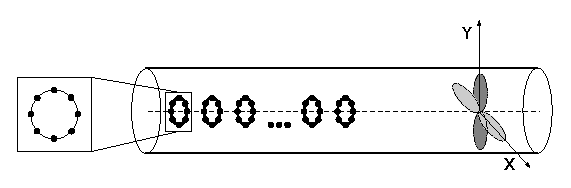
\includegraphics[width=1\linewidth]{./images/logging_tool_scheme.eps}
	\caption{\footnotesize Схема модельных измерений.}
	\label{fig:measurement_scheme}
\end{figure}

Матрица измерений $\mathbf{R}$, полученная при моделировании, не является строго симметричной из-за наличия шума в сигналах. Чем меньше отношение $E_{rel}$ суммы квадратов значений недиагональных компонент матрицы $\mathbf{D}$, полученной после преобразования матрицы измерений, тем лучше работает алгоритм диагонализации и тем достовернее значения полученных углов. При обработке эталонных имитируемых измерений в цилиндрической скважине величина $E_{rel}$ имеет значения порядка $10^{-7}$; угол $\theta$ совпадает с заданным модельным значением до десятых долей градуса. Эти значения имеют порядок погрешности численного метода и алгоритма обработки. 

Для оценки влияния несимметричности формы скважины на результат работы Alford rotation и его неортогонального обобщения были рассмотрены примеры эллиптических скважин в ТИ породах  Bakken Shale и Cotton Valey Shale. Обе породы относятся к классу глинистых сланцев и имеют скорость распространения поперечных волн, превышающую скорость звука в жидкости в скважине (т. н. быстрые породы). Значение упругих постоянных материалов приведены в табл.~\ref{tab:properties}. Ось симметрии ТИ породы наклонена по отношению к оси скважины под углом 90\textdegree (горизонтальная трансверсальная изотропия), искомый угол поворота оси симметрии в плоскости поперечного сечения скважины равен $\theta = 45$\textdegree. В расчётах использовались скважины c размерами полуосей $12,70 \times 10,16$ см и $15 \times 10$ см. Модельные осредненные сигнатуры давления с приемников для измерения XX представлены на рис.~\ref{fig:disp_curves_all},\textit{а,б}.
%Полное описание рассматриваемых моделей можно найти в таблице \ref{tab:models_description}. 

Оба алгоритма на исходных модельных данных дают примерно одинаковые результаты для углов поворота (табл.~\ref{tab:std_process_results}). Полученные главные направления почти ортогональны, но значительно отличаются от заданных в модели значений 45\textdegree \ и -45\textdegree. При этом в недиагональных компонентах преобразованных матриц измерений остаётся достаточно мало энергии -- от 1 до 3\%. Такой результат для матрицы из полевых данных можно считать достаточно хорошим с практической точки зрения, но при этом вычисленные направления главных осей анизотропной породы не совпадают с физическими.

В \cite{Seroices2010} было показано , что в эллиптических скважинах на низких частотах форма поперечного сечения почти не оказывает влияния на распространение волн, а определяется свойствами породы. Рассмотрим вопрос, как результат обработки зависит от частотного спектра приходящего сигнала. Особенностью распространения дипольных колебаний в скважине является большая дисперсия. С помощью модифицированного метода Прони \cite{Ekstrom1995}, были построены дисперсионные кривые для гармоник исходного сигнала с наиболее высокой амплитудой (рис. \ref{fig:disp_curves_all}-в,г). В моделируемых задачах они соответствуют двум главным дипольным модам. %. Аналогичные кривые также были построены по результатам расчётов полуаналитическим методом конечных элементов (SAFE) и нанесены на графики для проверки точности. 
По этим кривым для каждой породы выделен диапазон низких частот, где скорость распространения волны почти постоянна и близка к одной из скоростей поперечных волн, а также диапазон высоких частот с достаточно постоянной скоростью распространения. 

Для выделенных таким образом частотных диапазонов сконструированы низкочастотные и высокочастотные фильтры с конечной импульсной характеристикой, которые были применены к исходным матрицам измерений перед обработкой. Полученные на основе фильтрованных данных оценки углов гораздо ближе к модельным значениям, чем значения от нефильтрованного сигнала (табл.~\ref{tab:filter_process_results}). На низких частотах при обработке фильтрованных данных наблюдается заметная неортогональность между направлениями поляризации дипольных мод. Применение высокочастотных фильтров, напротив приводит к почти полностью ортогональному результату, близкому к направлениям осей эллипса. 

\begin{figure}[h]
	\centering
	\begin{minipage}{0.49\linewidth}
		\centering %\textbf{Bakken Shale}
		\psfragfig[width=0.49\linewidth,crop=pdfcrop]{./images/nonorth_alford/el15x10_BS_HTI_45_Drot1} \\
		а)
	\end{minipage}
	\begin{minipage}{0.49\linewidth}
		\centering %\textbf{Cotton Valey Shale}
		\psfragfig[width=0.49\linewidth,crop=pdfcrop]{./images/nonorth_alford/el15x10_CS_HTI_45_Drot1} \\
		б)
	\end{minipage}
	\begin{minipage}{0.49\linewidth}
		\centering %\textbf{Bakken Shale}
		\psfragfig[width=0.49\linewidth,crop=pdfcrop]{./images/nonorth_alford/el15x10_HTI_BS_f45_disp_modes+SAFE} \\
		в)
	\end{minipage}
	\begin{minipage}{0.49\linewidth}
		\centering %\textbf{Cotton Valey Shale}
		\psfragfig[width=0.49\linewidth,crop=pdfcrop]{./images/nonorth_alford/el15x10_HTI_CS_f45_disp_modes+SAFE_new} \\
		г)
	\end{minipage}
	\caption{\footnotesize Исходные сигнатуры давления для измерения ХХ, смоделированные в SEM, а также дисперсионные кривые для двух дипольных мод в эллиптических скважинах ($15 \times 10$ см) в породах Bakken Shale (а,в) и Cotton Valey Shale (б,г). Дисперсионные кривые на графиках независимо получены модифицированным методом Прони (на основе данных моделирования SEM) и методом SAFE. }
	\label{fig:disp_curves_all}
\end{figure}

\section{Сравнение решений SAFE с результатами обработки решений SEM}
\label{safe_comparison}

Полуаналитический метод конечных элементов использует представление решения для волнового поля в скважине волн в виде суммы мод. Основная энергия в волне, возбуждаемой дипольным источником, содержится в дипольных модах, поэтому из всего набора собственных векторов выбраны те, которые соответствуют именно этим колебаниям. Градиент значений собственного вектора в скважине позволяет получить направление преимущественного колебания частиц на некоторой частоте. В породах, выбранных для моделирования, эти направления существенно меняются в районе от 4 до 6 кГц \cite{Zharnikov2015}. Но в зонах пропускания используемых низкочастотных и высокочастотных фильтров изменения направлений градиентов собственных векторов невелики. Для сравнения с результатами обработки Alford rotation (табл.~\ref{tab:filter_process_results}) выбраны собственные вектора для дипольных мод на частоте, соответствующей максимумам энергии в спектре фильтрованных данных (см. рис.~\ref{fig:comparison_safe_all}).

На представленных изображениях хорошо видна неортогональность градиентов собственных векторов дипольных мод на низких частотах. Заметим также, что в этом частотном диапазоне результат практически не отличается для двух выбранных геометрий скважин. Если сопоставить направления градиентов с углами, полученными с помощью Alford rotation, то наиболее близкими к ним окажутся результаты, полученные неортогональным алгоритмом. Отсутствие точного соответствия объясняется более широким спектром исследуемого сигнала, в котором характер колебаний может быть лишь приближен собственными векторами дипольных мод на одной частоте. Тем не менее представленное сравнение объясняет почему полученные алгоритмом Alford rotation направления не совпадают с заданной в изначальной модели ориентацией оси симметрии трансверсально-изотропной породы. Этот пример демонстрирует ограниченность применения классического подхода оценки главных направлений ТИ породы в задачах такого типа. 

%Отметим, что близкие к 45\textdegree \ значения угла классического ортогонального Alford rotation являются лишь случайным совпадением осредненных реальных поляризаций мод на этих частотах с заданным значением в модели. В пользу этого утверждения говорит факт, что энергия недиагональных компонент при ортогональной обработке достаточно велика - до 10\% (см. Таблицу \ref{tab:filter_process_results}). 

Результаты обработки нефильтрованного сигнала в рассмотренных задачах, как следует из данных таблиц, в целом дают близкие значения к результатам обработки сигнала после применения высокочастотного фильтра. Интересно, что при этом поляризация мод почти ортогональна, но не совпадает с направлениями полуосей эллипса поперечного сечения скважины. При увеличении степени эллиптичности ствола это различие уменьшается. Таким образом, даже при корректной (с точки зрения диагонализации матрицы измерений) работе алгоритма полученное значение угла на направление главной оси анизотропного материала может не отвечать ни физическим свойствам породы, ни геометрической ориентации скважины. 

\begin{figure}[h]
\centering
\renewcommand{\arraystretch}{1.5}
\begin{tabular*}{1\textwidth}{c|cc|cc|}
\cline{2-5}
&\multicolumn{2}{c|}{\textbf{Bakken Shale ($12.70 \times 10.16$)}} &\multicolumn{2}{c|}{\textbf{Bakken Shale ($15.00 \times 10.00$)}}\\ 
\begin{minipage}{0.02\textwidth}
\rotatebox{90}{\footnotesize \textit{Дипольная мода 1}} 
\end{minipage}&
\begin{minipage}{0.22\textwidth}
	\psfragfig[width=0.23\textwidth,crop=pdfcrop]{./images/SAFE/SAFE_BS_10x8_HTI_45/P_s_3_3kHz}		
\end{minipage}&
\begin{minipage}{0.22\textwidth}
	\psfragfig[width=0.23\textwidth,crop=pdfcrop]{./images/SAFE/SAFE_BS_10x8_HTI_45/P_s_5_5kHz}		
\end{minipage}&
\begin{minipage}{0.22\textwidth}
	\psfragfig[width=0.23\textwidth,crop=pdfcrop]{./images/SAFE/SAFE_BS_15x10_HTI_45/P_s_3_3kHz}		
\end{minipage}&
\begin{minipage}{0.22\textwidth}
	\psfragfig[width=0.23\textwidth,crop=pdfcrop]{./images/SAFE/SAFE_BS_15x10_HTI_45/P_s_5_5kHz}		
\end{minipage}\\ 
%& & & & \\
\begin{minipage}{0.02\textwidth}
\rotatebox{90}{\footnotesize \textit{Дипольная мода 2}} 
\end{minipage} &
\begin{minipage}{0.22\textwidth}
	\psfragfig[width=0.23\textwidth,crop=pdfcrop]{./images/SAFE/SAFE_BS_10x8_HTI_45/P_a_3_3kHz}		
\end{minipage} &
\begin{minipage}{0.22\textwidth}
	\psfragfig[width=0.23\textwidth,crop=pdfcrop]{./images/SAFE/SAFE_BS_10x8_HTI_45/P_a_5_5kHz}		
\end{minipage} &
\begin{minipage}{0.22\textwidth}
	\psfragfig[width=0.23\textwidth,crop=pdfcrop]{./images/SAFE/SAFE_BS_15x10_HTI_45/P_a_3_3kHz}		
\end{minipage} &
\begin{minipage}{0.22\textwidth}
	\psfragfig[width=0.23\textwidth,crop=pdfcrop]{./images/SAFE/SAFE_BS_15x10_HTI_45/P_a_5_5kHz}		
\end{minipage} \\ 
& \footnotesize НЧФ, 3.29 кГц & \footnotesize ВЧФ, 5.53 кГц & \footnotesize НЧФ, 3.29 кГц & \footnotesize ВЧФ, 5.53 кГц \\ \cline{2-5}
\end{tabular*} \\
{а)} \\
\quad \\
\begin{tabular*}{1\textwidth}{c|cc|cc|}
\cline{2-5}
&\multicolumn{2}{c|}{\textbf{Cotton Valey Shale ($12.70 \times 10.16$)}} &\multicolumn{2}{c|}{\textbf{Cotton Valey Shale ($15.00 \times 10.00$)}}\\
\begin{minipage}{0.02\linewidth}
	\rotatebox{90}{\footnotesize\textit{Дипольная мода 1}} 
\end{minipage}&
\begin{minipage}{0.22\linewidth}
	\psfragfig[width=0.22\linewidth,crop=pdfcrop]{./images/SAFE/SAFE_CS_10x8_HTI_45/P_s_3_0kHz}		
\end{minipage}&
\begin{minipage}{0.22\linewidth}
	\psfragfig[width=0.22\linewidth,crop=pdfcrop]{./images/SAFE/SAFE_CS_10x8_HTI_45/P_s_7_2kHz}		
\end{minipage}&
\begin{minipage}{0.22\linewidth}
	\psfragfig[width=0.22\linewidth,crop=pdfcrop]{./images/SAFE/SAFE_CS_15x10_HTI_45/P_s_3_0kHz}		
\end{minipage}&
\begin{minipage}{0.22\linewidth}
	\psfragfig[width=0.22\linewidth,crop=pdfcrop]{./images/SAFE/SAFE_CS_15x10_HTI_45/P_s_7_2kHz}		
\end{minipage} \\
\begin{minipage}{0.02\linewidth}
	\rotatebox{90}{\footnotesize\textit{Дипольная мода 2}} 
\end{minipage}&
\begin{minipage}{0.22\linewidth}
	\psfragfig[width=0.22\linewidth,crop=pdfcrop]{./images/SAFE/SAFE_CS_10x8_HTI_45/P_a_3_0kHz}		
\end{minipage}&
\begin{minipage}{0.22\linewidth}
	\psfragfig[width=0.22\linewidth,crop=pdfcrop]{./images/SAFE/SAFE_CS_10x8_HTI_45/P_a_7_2kHz}		
\end{minipage}&
\begin{minipage}{0.22\linewidth}
	\psfragfig[width=0.22\linewidth,crop=pdfcrop]{./images/SAFE/SAFE_CS_15x10_HTI_45/P_a_3_0kHz}		
\end{minipage}&
\begin{minipage}{0.22\linewidth}
	\psfragfig[width=0.22\linewidth,crop=pdfcrop]{./images/SAFE/SAFE_CS_15x10_HTI_45/P_a_7_2kHz}		
\end{minipage}\\
& \footnotesize НЧФ, 3.03 кГц & \footnotesize ВЧФ, 7.17 кГц & \footnotesize НЧФ, 3.03 кГц & \footnotesize ВЧФ, 7.17 кГц \\ \cline{2-5}
\end{tabular*}
\\
{б)} \\
\quad \\
\renewcommand{\arraystretch}{1.0}
\footnotesize
\begin{tabular*}{\textwidth}{@{\extracolsep{\fill} }crccc}
& 						 	& \tikz \draw (0,0) -- (1cm,0);  	& \tikz \draw[dashed] (0,0) -- (1cm,0);  	& \tikz \draw[very thick,dashdotted] (0,0) -- (1cm,0); \\
& Результаты обработки 		& \textit{ортогональный} 			& \textit{ортогональный} 					& \textit{неортогональный}    			\\
& Alford rotation:			& \textit{без фильтрации}		 	& \textit{с фильтрацией} 					& \textit{с фильтрацией} 	\\
\end{tabular*}
\renewcommand{\arraystretch}{1.0}
\caption{ \footnotesize Сравнение результатов обработки фильтрованных данных измерений и значений собственных векторов дипольных мод на частоте, соответствующей максимуму энергии в спектре сигнала, в породе Bakken Shale (а) и Cotton Valey Shale (б). Распределение давления (собственный вектор) в сечении скважины показано серым цветом, черные участки соответствуют максимальному и минимальному значениям. НЧФ и ВЧФ соответствуют низкочастотной (НЧФ) и высокочастотной (ВЧФ) фильтрации, применённой к исходным данным.}
\normalsize
\label{fig:comparison_safe_all}
\end{figure}

\section{Заключение}
Приведённые в работе расчёты показывают, что деформация ствола скважины может значительно влиять на результат работы алгоритмов определения главных направлений анизотропной породы в случаях, когда характерные направления деформации и анизотропии не совпадают. Изменение формы приводит к появлению неортогональности направлений поляризации дипольных мод, а также к зависимости этих направлений от частотного спектра распространяющейся волны. Таким образом, неортогональная модификация алгоритма Alford rotation позволяет выявить на этапе обработки данных признаки возможного несоответствия результата физическим свойствам породы.  

Применение частотных фильтров, сужающих спектр исходных данных измерений в низкочастотную область, позволяет получить более точные оценки главных направлений. Рассмотренные в работе примеры демонстрируют, что ортогональность направлений, полученных в ходе обработки, не является критерием корректности результата -- необходимо отсутствие значительной зависимости получаемого ответа от параметров фильтра и ширины временного окна. Недостатком обработки измерений в низкочастотной области является, очевидно, резкое падение энергии приходящего сигнала по сравнению с естественными шумами.

Результаты обработки каротажных измерений в быстрых породах ортогональным и неортогональным методами, основанными на диагонализации матрицы измерений, определяются поляризацией нормальных мод на высоких частотах. Данный вывод является достаточно интересным, так как, несмотря на продемонстрированную сильную частотную зависимость направлений собственных векторов дипольных мод, поперечная поляризация волн всего сигнала в целом существует и хорошо согласуется с высокочастотными решениями, полученными SAFE. 

%Важным результатом данной работы является оценка точности работы упомянутых алгоритмов, а также демонстрация возможного существования ортогонально поляризованных волн в быстрых породах,  не связанных однозначно с одним из факторов. Для дипольных мод на средних частотах существует область с достаточно резкой сменой направлений поляризации, которая однако не имеет определяющего значения для работы алгоритма, так как спектр используемых источников значительно шире.

Приведённый материал демонстрирует возможности спектральных алгоритмов, построенных на основе полуаналитического метода конечных элементов, для анализа и интерпретации особенностей волнового поля в скважинах. Высокая скорость расчётов, а также возможность распространения метода на среды с более общим типом анизотропии, затуханием и начальными напряжениями открывает широкие перспективы применения рассмотренной методики для улучшения качества обработки каротажных измерений. 

Работа выполнена на базе Московского научного центра Шлюмберже.

\begin{table}[H]
	\footnotesize
	%\centering
	\caption{Параметры упругих анизотропных материалов}
	\renewcommand{\arraystretch}{1.5}
	\begin{tabularx}{\textwidth}{|C|c|c|c|c|c|c|c|}
		\hline \multirow{2}{*}{Название}  & Плотность, & \multicolumn{6}{c|}{Модули упругости, ГПа} \\ 
		\cline{3-8}  & кг/м$^3$ & $C_{11}$ & $C_{12}$ & $C_{13}$ & $C_{33}$ & $C_{44}$ & $C_{66}$ \\ \hline
		\hline Cotton Valey Shale & 2640 & 74.73 & 14.75 & 25.29 & 58.84 & 22.05 & 29.99 \\ 
		\hline Bakken Shale & 2230 & 40.9 & 10.3 & 8.5 & 26.9 & 10.5 & 15.3 \\ 
		\hline 
	\end{tabularx} 
	\label{tab:properties}
	\renewcommand{\arraystretch}{1.0}
\end{table}

\begin{table}[h]
	\footnotesize
	%\centering
	\caption{Результаты обработки исходных данных алгоритмами Alford rotation}
	\renewcommand{\arraystretch}{1.5}
	\begin{tabularx}{\textwidth}{|X|rr|rr|r|rr|}
		\hline	
		&\multicolumn{1}{c}{$\theta_1^o$} & \multicolumn{1}{c|}{$\theta_1^n$} & \multicolumn{1}{c}{$\theta_2^o$} & \multicolumn{1}{c|}{$\theta_2^n$} & \multicolumn{1}{c|}{$\Delta\theta^n$}& \multicolumn{1}{c}{$E_{rel}^o, \%$} & \multicolumn{1}{c|}{$E_{rel}^n, \%$} \\ \hline
		\hline Bakken Shale ($12.70 \times 10.16$) & 15.6 & 14.7 & -74.4 & -73.9  & 1.4  & 3.0 & 3.0 \\
		\hline Bakken Shale ($15.00 \times 10.00$) & 8.4 & 8.1 & -81.6 & -81.6 & 0.3 & 1.7 & 1.7 \\
		\hline Cotton Valey Shale ($12.70 \times 10.16$) & 3.3 & 3.0 & -86.7 & -86.7  & 0.3 & 0.8 & 0.8 \\ 
		\hline Cotton Valey Shale ($15.00 \times 10.00$) & 1.6 & 1.8 & -88.4 & -88.4  & 0.0  & 0.6 & 0.6 \\	   
		\hline
	\end{tabularx} 
	\begin{flushleft}
		Примечание. Здесь $\theta_1^o,\theta_2^o$ и $\theta_1^n,\theta_2^n$ соответствуют результатам, полученным ортогональной и неортогональной версией алгоритма; величина $E_{rel}$ обозначает отношение энергии недиагональных компонент матрицы измерений к полной энергии. 
	\end{flushleft}
	\label{tab:std_process_results}
	\renewcommand{\arraystretch}{1.0}
\end{table}

\begin{table}[h]
	\footnotesize
	\centering
	\caption{Результаты обработки данных после применением фильтров}
	\renewcommand{\arraystretch}{1.5}
	\begin{tabularx}{\textwidth}{|X|rr|rr|r|rr|}
		\hline
		&\multicolumn{1}{c}{$\theta_1^o$} & \multicolumn{1}{c|}{$\theta_1^n$} & \multicolumn{1}{c}{$\theta_2^o$} & \multicolumn{1}{c|}{$\theta_2^n$} & \multicolumn{1}{c|}{$\Delta\theta^n$}& \multicolumn{1}{c}{$E_{rel}^o, \%$} & \multicolumn{1}{c|}{$E_{rel}^n, \%$} \\ \hline
		\hline	\textbf{Bakken Shale ($12.70 \times 10.16$)} & \textbf{15.6} & \textbf{14.7} & \textbf{-74.4}  & \textbf{-73.9}  & \textbf{1.4}  & \textbf{3.0} & \textbf{3.0} \\
		-//-//- с НЧФ & 49.4 & 40.5 & -40.6 & -35.4  & 14.1 & 2.0 & 1.2\\
		-//-//- с ВЧФ & 14.0 & 13.3 & -76.0 & -75.6  & 1.2 & 0.4 & 0.4\\
		\hline	\textbf{Bakken Shale ($15.00 \times 10.00$)} & \textbf{8.4} & \textbf{8.1} & \textbf{-81.6}  & \textbf{-81.6} & \textbf{0.3}  & \textbf{1.7} & \textbf{1.7} \\
		-//-//- с НЧФ & 41.2 & 25.7 & -48.8 & -32.0  & 32.3 & 22.1 & 12.0\\
		-//-//- с ВЧФ & 7.5 & 10.2 & -82.5 & -82.6  & 2.8 & 1.1 & 1.0\\
		\hline	\textbf{Cotton Valey Shale ($12.70 \times 10.16$)} & \textbf{3.3} & \textbf{3.0} & \textbf{-86.7}  & \textbf{-86.7}  & \textbf{0.3}  & \textbf{0.8} & \textbf{0.8}\\
		-//-//- с НЧФ & 48.4 & 39.7 & -41.6 & -35.5  & 14.8  & 9.7 & 7.0 \\
		-//-//- с ВЧФ & 2.8 & 3.3 & -87.2 & -87.4  & 0.7  & 0.5 & 0.5\\	
		\hline	\textbf{Cotton Valey Shale ($15.00 \times 10.00$)} & \textbf{1.6} & \textbf{1.8} & \textbf{-88.4}  & \textbf{-88.4}  & \textbf{0.00}  & \textbf{0.6} & \textbf{0.6} \\
		-//-//- с НЧФ & 6.0 & 7.7 & -84.0 & -56.6  & 25.7  & 7.9 & 7.3 \\
		-//-//- с ВЧФ & 1.5 & 2.0 & -88.5 & -88.7  & 0.7  & 1.8 & 1.8\\		
		\hline	
	\end{tabularx} 
	\begin{flushleft}
		Примечание. Здесь $\theta_1^o,\theta_2^o$ и $\theta_1^n,\theta_2^n$ соответствуют результатам, полученным ортогональной и неортогональной версией алгоритма. Величина $E_{rel}$ обозначает отношение энергии недиагональных компонент матрицы измерений к полной энергии. НЧФ и ВЧФ соответствуют низкочастотной (НЧФ) и высокочастотной (ВЧФ) фильтрации, применённой к исходным данным.
	\end{flushleft}
	\label{tab:filter_process_results}
	\renewcommand{\arraystretch}{1.0}
\end{table}

\clearpage

%\bibliography{./library/library}
%\include{include/var_bibliography_link}

\bibliographystyle{gost2008s}
%\bibliography{c:/Users/German/Documents/TeX_Library/library}
\bibliography{d:/Documents/Workfiles/Literature/TeX_Library/library}


%\bibliographystyle{plainnat_no_url}



\end{document} 